\documentclass[10pt,a4paper]{article}
\usepackage[margin=2.2cm]{geometry}
\usepackage{amsmath,amssymb,graphicx,booktabs,braket}
\usepackage[hidelinks]{hyperref}
\usepackage[font=small,labelfont=bf]{caption}
\usepackage{microtype}
\graphicspath{{../figures/}}

\title{\textbf{How much gate-synthesis error can Rodeo eigenvalue estimation tolerate?}\\[2pt]
\large Clifford+T compilation of transverse-field Ising dynamics}
\author{Minka Dubourg}
\date{March 2025}

\begin{document}
\maketitle

\begin{abstract}
\noindent
The Rodeo algorithm estimates eigenvalues by filtering an initial state through randomly timed, ancilla-controlled time evolutions. On fault-tolerant hardware with a Clifford+T gate set, every rotation in that evolution must be compiled into a finite gate sequence. Each compiled rotation then carries a synthesis error~$\varepsilon$ and a cost in T gates.

We study this trade-off for the transverse-field Ising chain. The compiler combines Ross--Selinger approximation with an independent re-implementation of Kliuchnikov--Maslov--Mosca exact synthesis that uses exact arithmetic in $\mathbb Z[1/\sqrt2,i]$. The Rodeo filter is evaluated from the eigendecomposition of the compiled Trotter step, and this evaluation is validated against circuit-level simulation to $10^{-9}$.

Three results follow.
(i) Correctly compiled evolution reproduces the exact spectrum, including the $\pm\sqrt5$ levels. Rounding the field rotation to the nearest diagonal Clifford+T gate instead silently removes the transverse field, and the spectra then look plausible but belong to the classical Ising model.
(ii) The eigenvalue error of the compiled evolution is the sum of a Trotter term $\propto dt^2$ and a synthesis term $\propto\varepsilon/dt$. Synthesis error therefore grows as the time step shrinks, and each~$\varepsilon$ has an optimal step.
(iii) Choosing that step matters for cost. For two spins, $\varepsilon=10^{-3}$ at $dt\approx0.14$ is four times more accurate than $\varepsilon=10^{-4}$ at $dt=0.005$, and needs 37 times fewer T gates per unit of simulated time.
\end{abstract}

\section{Introduction}
Many quantum algorithms need eigenvalues of a Hamiltonian $H$. The Rodeo algorithm~\cite{rodeo} is a simple way to obtain them. Each cycle prepares an ancilla in $(\ket0-\ket1)/\sqrt2$, applies $e^{-iHt_k}$ controlled on the ancilla, applies a phase $e^{iEt_k}$, then a Hadamard, and keeps the run if the ancilla reads~1. For an eigenstate with energy $\lambda$, the success probability of one cycle is $\cos^2\!\big((E-\lambda)t_k/2\big)$. With $N$ cycles at random times $t_k\sim\mathcal N(0,t_\mathrm{RMS}^2)$, the product of these factors acts as a filter that passes only states with $\lambda\approx E$, with a resolution of about $1/t_\mathrm{RMS}$.

On error-corrected hardware the native gates are Clifford gates plus the T gate, and T gates dominate the cost. The continuous rotations in a Trotterised $e^{-iHt}$ must therefore be \emph{synthesised}. Two tools do this:
\begin{itemize}
\item Ross--Selinger approximation~\cite{ross} finds a Clifford+T unitary within operator-norm distance $\varepsilon$ of $R_z(\theta)$, using about $3\log_2(1/\varepsilon)$ T gates. This is far fewer than the general-purpose Solovay--Kitaev algorithm~\cite{sk}, whose sequence length grows polylogarithmically with a larger exponent.
\item Exact synthesis~\cite{kmm} then turns that unitary into a gate word.
\end{itemize}
This report asks how the synthesis precision, the Trotter step and the T-count interact with the energies that Rodeo reports.

\section{Methods}
\paragraph{Model.} We study the open transverse-field Ising chain $H=-J\sum_k Z_kZ_{k+1}+h\sum_k X_k$ with $J=h=1$. For $n=2$ its spectrum is $\{-\sqrt5,-1,1,\sqrt5\}$. The evolution uses first-order Trotter steps,
\[
W(dt)=\prod_k R_{zz}^{(k,k+1)}(-2J\,dt)\,\prod_k R_x^{(k)}(2h\,dt),
\]
with $R_{zz}=\mathrm{CNOT}\,(I\otimes R_z)\,\mathrm{CNOT}$ and $R_x=H R_z H$. Every rotation is thus an $R_z$, and there are $R=2n-1$ of them per step.

\paragraph{Compilation.} Each $R_z(\theta)$ is approximated to precision $\varepsilon$ with the Ross--Selinger algorithm, using the \texttt{pygridsynth} implementation~\cite{pygridsynth}. The resulting word is converted to an exact $2\times2$ matrix over $\mathbb Z[1/\sqrt2,i]$. That matrix is then re-synthesised with our own implementation of exact synthesis~\cite{kmm}:
\begin{itemize}
\item while $s=\mathrm{sde}(|U_{00}|^2)\ge4$, apply the step $U\mapsto HT^kU$ that lowers $s$ by one;
\item look up the remainder in a table of all 1664 unitaries with $s\le3$, built by breadth-first search.
\end{itemize}
All arithmetic is exact: elements are stored as $(a+b\omega+c\omega^2+d\omega^3)/\sqrt2^{\,k}$ with integer coefficients. Each re-synthesised word reproduces its input exactly, including the global phase, and has the same (optimal) T-count. The global phase matters because Rodeo uses \emph{controlled} evolution, where a phase error becomes a shift in energy.

As a baseline, we also consider rounding $\theta$ to the nearest multiple of $\pi/4$. This is equivalent to searching only over diagonal Clifford+T gates.

\paragraph{Rodeo filter.} Each Rodeo time is an integer number of Trotter steps, $t_k=n_kdt$. If the compiled step $W$ has orthonormal eigenvectors $v_j$ and eigenphases $\phi_j$, the success probability is
\[
P(E)=\sum_j |\braket{v_j|\psi_0}|^2\prod_{k=1}^{N}\cos^2\!\Big(\frac{E\,n_kdt+\phi_j n_k}{2}\Big),
\]
averaged over 400 draws of the $n_k$, with $N=10$ cycles and $t_\mathrm{RMS}=5$. This expression equals a noise-free statevector simulation of the full ancilla circuit, to $10^{-9}$ in our tests, but it is far cheaper to evaluate. The spectral error is measured on the effective Hamiltonian $W=e^{-iH_\mathrm{eff}dt}$ as $\max_j|E_j(H_\mathrm{eff})-E_j(H)|$.

\section{Results}
\subsection{Compiled evolution recovers the spectrum; diagonal rounding removes the field}
Figure~\ref{fig:spectra} shows Rodeo spectra for four initial states. With exact rotations, and equally with Ross--Selinger rotations at $\varepsilon=10^{-3}$, the peaks sit at the exact eigenvalues and their heights equal the overlaps $|\braket{v_j|\psi_0}|^2$.

Diagonal rounding behaves differently. The field rotation $R_x(2h\,dt)$ has an angle of only $0.2$ at $dt=0.1$, which rounds to the identity, so the compiled evolution is that of $-JZ_1Z_2$ alone. The resulting spectra are internally consistent:
\begin{itemize}
\item peaks at $\pm1$ with weights $\tfrac12$ for $\ket{++}$;
\item a single peak at $-1$ for $\ket{00}$;
\item a single peak at $+1$ for $\ket{01}$.
\end{itemize}
These would pass a sanity check against the wrong model. Only the antisymmetric state $\ket{+-}$, whose overlaps happen to be identical for the two models, cannot distinguish them.

\begin{figure}[t]\centering
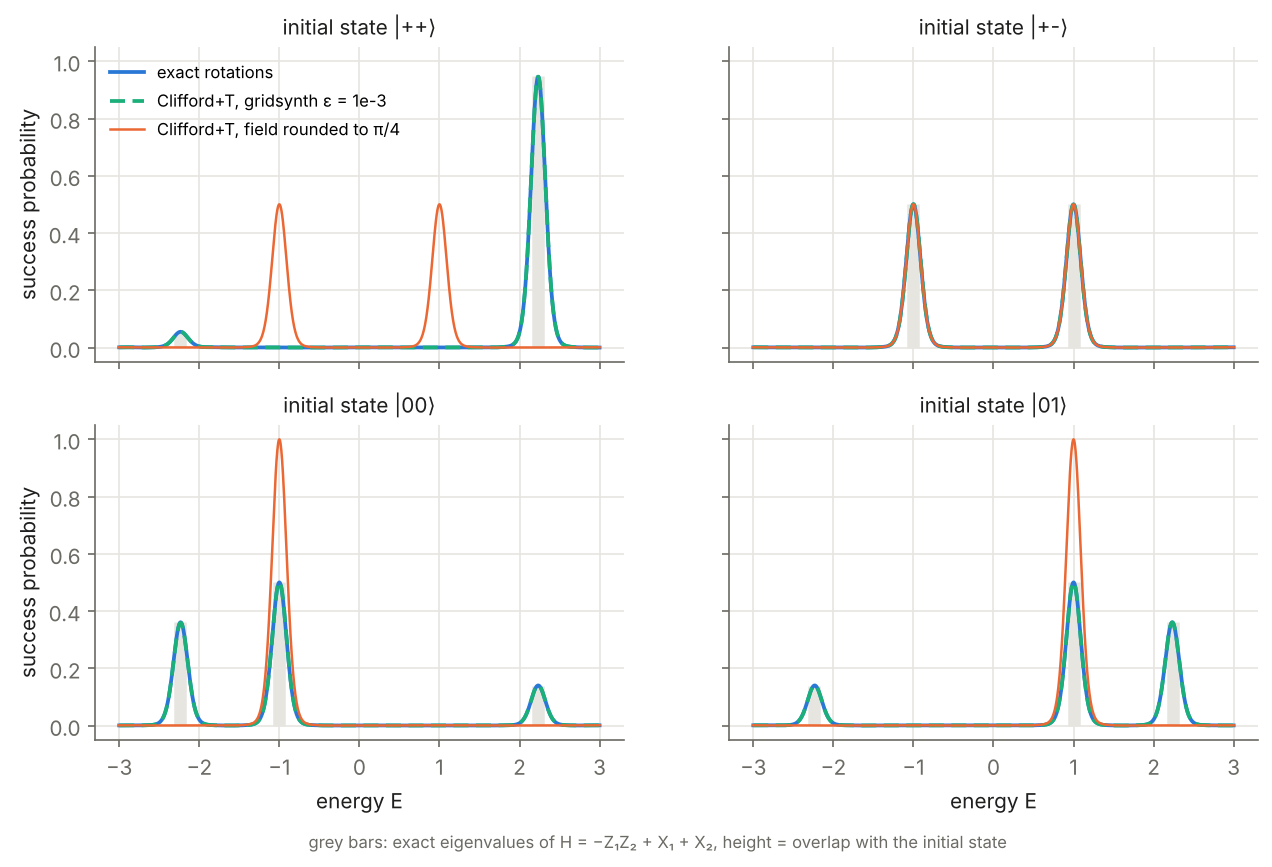
\includegraphics[width=0.92\textwidth]{spectra.png}
\caption{Rodeo spectra for $n=2$, $dt=0.1$. Grey bars: exact eigenvalues, with height equal to the overlap with the initial state. Exact and Ross--Selinger-compiled evolutions overlap. Rounding the field rotation to a multiple of $\pi/4$ reproduces the spectrum of $-Z_1Z_2$.}\label{fig:spectra}
\end{figure}

\subsection{Error budget: Trotter error falls with $dt$, synthesis error rises}
Each compiled rotation differs from its target by at most $\varepsilon$, so one step deviates from the exact Trotter step by at most $R\varepsilon$. Because the same angles repeat at every step, these errors add coherently: over a time $t$ there are $t/dt$ steps, and the effective-Hamiltonian error grows like $R\varepsilon/dt$. The Trotter error of the first-order product formula on the eigenvalues scales as $c\,dt^2$; we fit $c=0.30$ for $n=2$ and $0.87$ for $n=4$, with exponent $2.01$.

The total error therefore has the U shape of Fig.~\ref{fig:budget}:
\begin{itemize}
\item at large $dt$, every curve follows the Trotter line;
\item at small $dt$, the error rises again as $\varepsilon/dt$, at 15--35\,\% of the worst-case bound $R\varepsilon/dt$;
\item for $\varepsilon\ge10^{-2}$ and $dt\lesssim10^{-2}$, the rotations become indistinguishable from the identity and the spectrum collapses.
\end{itemize}
Minimising $R\varepsilon/dt+c\,dt^2$ gives an optimal step $dt^*\approx(R\varepsilon/2c)^{1/3}$ and a smallest achievable error that scales as $\varepsilon^{2/3}$. The numerical optima follow this scaling within a factor of about three, the scatter coming from the angle-to-angle variation of the synthesis error.

\begin{figure}[t]\centering
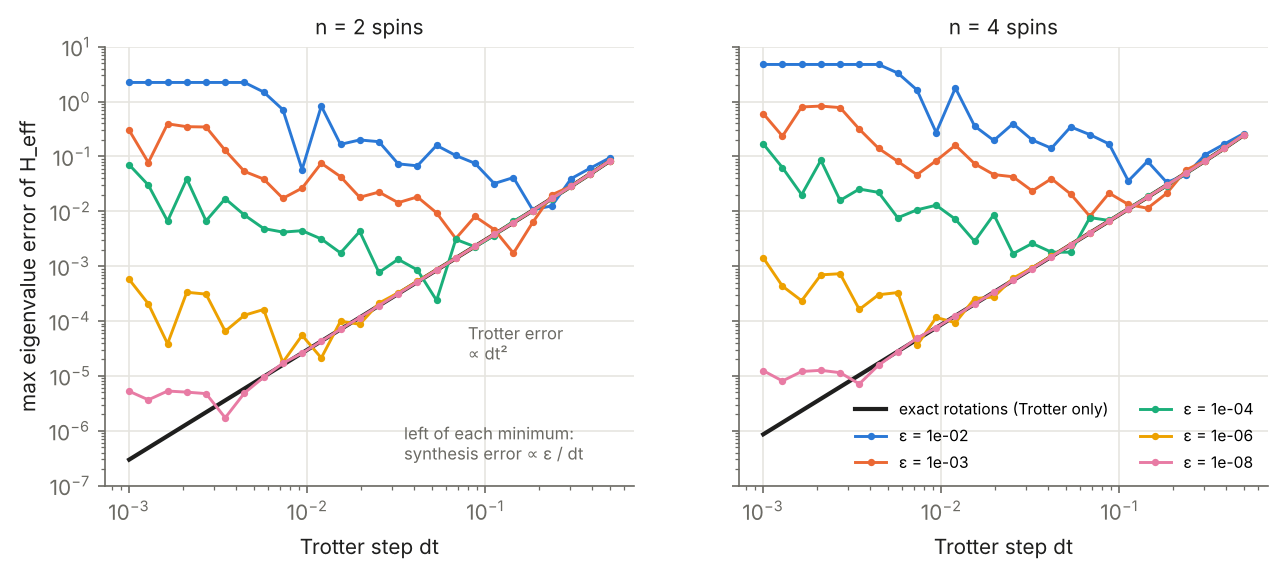
\includegraphics[width=\textwidth]{error_budget.png}
\caption{Maximum eigenvalue error of the compiled Trotter evolution against the step $dt$, for several synthesis precisions $\varepsilon$. Black: exact rotations (Trotter error only).}\label{fig:budget}
\end{figure}

\subsection{Cost of accuracy}
The T-count per unit of simulated time is $R\cdot T(\varepsilon)/dt$ with $T(\varepsilon)\approx3\log_2(1/\varepsilon)$. Small steps are therefore expensive twice over: they need more steps, and each step needs a tighter $\varepsilon$ to keep the synthesis term down. Figure~\ref{fig:cost} plots every $(\varepsilon,dt)$ choice for $n=2$. The configurations with $dt\approx0.005$ (open squares) are dominated by larger steps at the same or lower cost.

For example, $\varepsilon=10^{-4}$ at $dt=0.005$ reaches an error of $6.9\times10^{-3}$ for about 26\,500 T gates per unit time. $\varepsilon=10^{-3}$ at $dt=0.14$ reaches $1.7\times10^{-3}$ for about 700. Figure~\ref{fig:pitfall} shows the effect on a Rodeo spectrum: with the same $\varepsilon=10^{-3}$, $dt=0.1$ reproduces the exact peaks, while $dt=0.005$ shifts the $\pm\sqrt5$ peaks outward by $0.08$, about 40\,\% of the peak width (FWHM $0.21$).

\begin{figure}[t]\centering
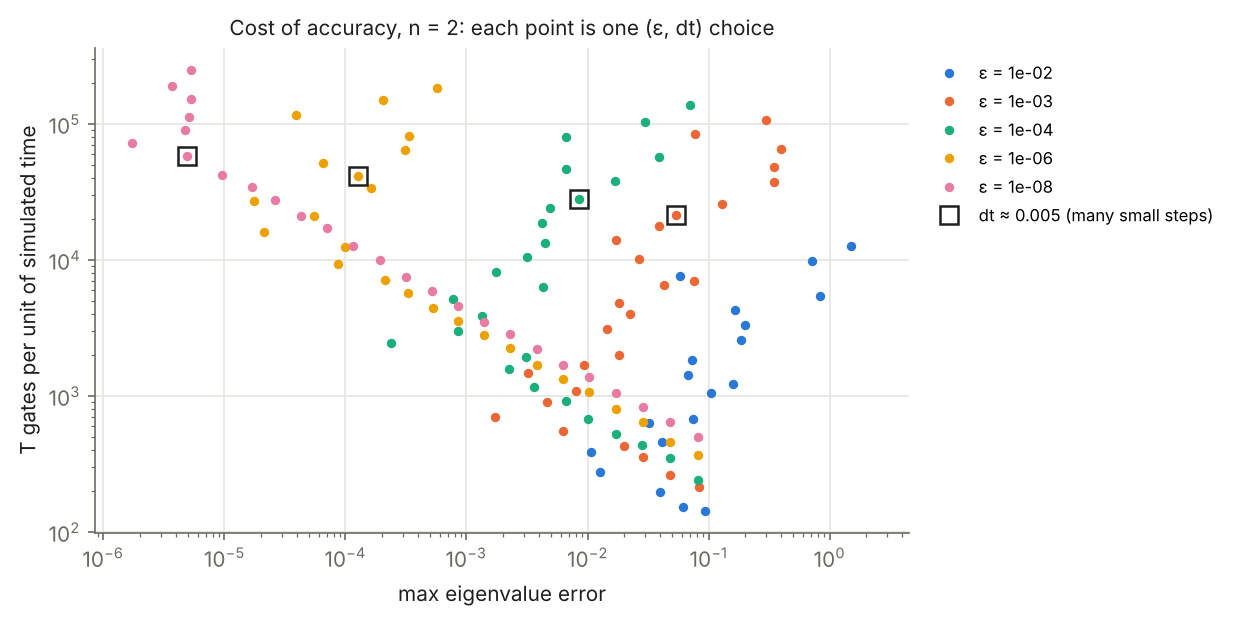
\includegraphics[width=0.72\textwidth]{cost_vs_accuracy.png}
\caption{T gates per unit of simulated time against the eigenvalue error, for all $(\varepsilon,dt)$ in Fig.~\ref{fig:budget} ($n=2$). Squares: $dt\approx0.005$.}\label{fig:cost}
\end{figure}

\begin{figure}[t]\centering
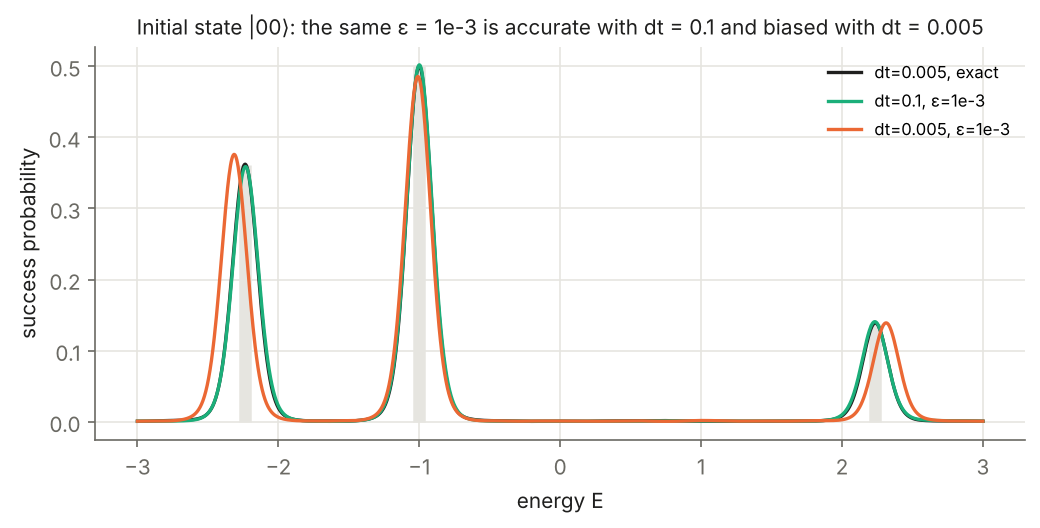
\includegraphics[width=0.78\textwidth]{step_size_pitfall.png}
\caption{Rodeo spectrum of $\ket{00}$ with synthesis precision $\varepsilon=10^{-3}$ at two step sizes, compared with exact rotations.}\label{fig:pitfall}
\end{figure}

\section{Discussion}
Two practical rules follow for Trotterised Rodeo, and plausibly for any phase-estimation-type algorithm built on compiled product formulas:
\begin{enumerate}
\item \textbf{Verify the compiled operator, not the spectrum.} A compiler that maps small angles to the identity produces clean, self-consistent spectra of a different Hamiltonian. Exact synthesis over $\mathbb Z[1/\sqrt2,i]$ makes it cheap to check every compiled word exactly against its target.
\item \textbf{Choose $\varepsilon$ and $dt$ together.} Synthesis error accumulates as $\varepsilon/dt$. Refining the time step without tightening $\varepsilon$ makes the energies \emph{worse}, and refining both costs T gates quadratically faster than necessary. Balancing the two terms gives $dt^*\propto\varepsilon^{1/3}$.
\end{enumerate}

\paragraph{Limitations.} The simulations are noise-free and use first-order Trotter steps on $n\le4$ spins. Higher-order formulas change the Trotter exponent and therefore the optimum. Controlled rotations are modelled as ideal controls of the compiled words; in practice each controlled $R_z$ costs two compiled rotations, which shifts the cost axis by a constant factor without changing the trade-off. Synthesis errors here are coherent because the same angles repeat at every step. Mixing several compiled approximations per angle could make them partially incoherent and reduce their accumulation, which is a natural next step.

\paragraph{Code.} All results are produced by \texttt{scripts/run\_experiments.py}. The test suite checks the exact-synthesis round trips, the Ross--Selinger error bound, and the agreement between the Rodeo filter formula and circuit simulation.

\begin{thebibliography}{9}\small
\bibitem{rodeo} K.~Choi, D.~Lee, J.~Bonitati, Z.~Qian, J.~Watkins. Rodeo algorithm for quantum computing. \textit{Phys. Rev. Lett.} 127, 040505 (2021).
\bibitem{ross} N.~J.~Ross, P.~Selinger. Optimal ancilla-free Clifford+T approximation of z-rotations. \textit{Quantum Inf. Comput.} 16, 901 (2016).
\bibitem{kmm} V.~Kliuchnikov, D.~Maslov, M.~Mosca. Fast and efficient exact synthesis of single-qubit unitaries generated by Clifford and T gates. \textit{Quantum Inf. Comput.} 13, 607 (2013).
\bibitem{sk} C.~M.~Dawson, M.~A.~Nielsen. The Solovay--Kitaev algorithm. \textit{Quantum Inf. Comput.} 6, 81 (2006).
\bibitem{pygridsynth} S.~Yamamoto, N.~Yoshioka. \texttt{pygridsynth}: a Python implementation of gridsynth. Python package, MIT licence.
\end{thebibliography}
\end{document}
